\documentclass[11pt,letterpaper]{article}

\usepackage[margin=1in]{geometry}
\usepackage{enumitem}
\usepackage{amsmath}
\usepackage{amssymb}
\usepackage{booktabs}
\usepackage{float}
\usepackage{needspace}
\usepackage{tikz}
\usetikzlibrary{decorations.pathmorphing, decorations.pathreplacing, calc, arrows.meta}
\usepackage[hidelinks]{hyperref}

% Answer space for students (no-ops in the solutions file)
\newcommand{\answerspace}[1]{\par\vspace{#1}}
\newcommand{\exampagebreak}{\newpage}

\newcommand{\pts}[1]{\textbf{[#1 pts]}}

% vector shorthands
\newcommand{\bn}{\mathbf{n}}
\newcommand{\be}{\hat{\mathbf{e}}_3}
\newcommand{\bw}{\boldsymbol{\omega}}
\newcommand{\bh}{\mathbf{h}}
\newcommand{\bJ}{\mathbf{J}}
\newcommand{\bQ}{\mathbf{Q}}

\title{16.07 Dynamics Midterm Exam}
\author{}
\date{}

\begin{document}

\maketitle
\vspace{-1.5cm}

\noindent\textbf{Instructions.} This exam has three parts: six short questions (Part I) and two longer problems (Parts II and III), for a total of 100 points. Show your work on the longer problems to ensure you receive partial credit. For multiple-choice questions, circle one or more answers as each problem instructs, and give a one-sentence justification.


% ==================================================================
\section*{Part I: Short Questions \hfill (30 points)}
% ==================================================================

\begin{enumerate}[label=\textbf{I.\arabic*}, leftmargin=*, itemsep=1em]

% ---------------- I.1 ----------------
\item \pts{5} \textbf{Stability from the potential.} Four frictionless, one-degree-of-freedom systems with coordinate $q$ have the potential energies sketched below near the equilibrium $q = 0$ (with $a > 0$ a constant).

\begin{center}
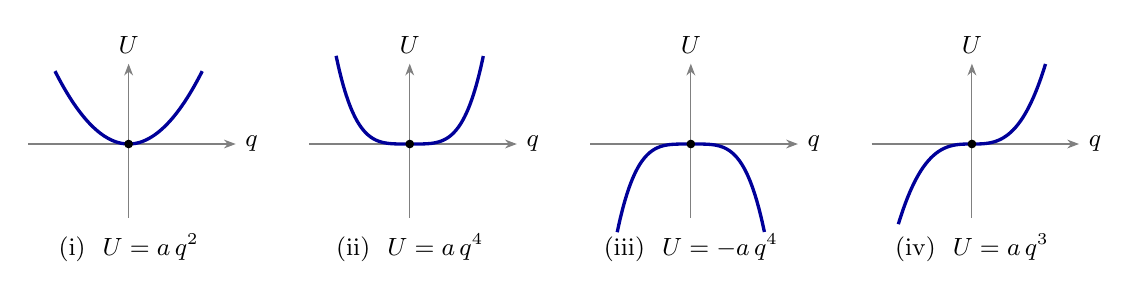
\begin{tikzpicture}[scale=0.85]
    \foreach \i/\lab/\form/\expr in {
        0/(i)/{U = a\,q^2}/{0.9*\x*\x},
        1/(ii)/{U = a\,q^4}/{0.9*\x*\x*\x*\x},
        2/(iii)/{U = -a\,q^4}/{-0.9*\x*\x*\x*\x},
        3/(iv)/{U = a\,q^3}/{0.9*\x*\x*\x}}{
        \begin{scope}[xshift=\i*4.2cm]
            \draw[-{Stealth[length=1.5mm]}, gray] (-1.5,0) -- (1.6,0) node[right, black, font=\small] {$q$};
            \draw[-{Stealth[length=1.5mm]}, gray] (0,-1.1) -- (0,1.2) node[above, black, font=\small] {$U$};
            \draw[very thick, blue!60!black, domain=-1.1:1.1, samples=60, smooth] plot (\x, {\expr});
            \filldraw (0,0) circle (1.6pt);
            \node[font=\small] at (0,-1.55) {\lab\ \ $\form$};
        \end{scope}
    }
\end{tikzpicture}
\end{center}

\begin{enumerate}[label=(\alph*)]
    \item Which of these equilibria are stable? Circle the label of each stable equilibrium in the sketches above.
    \item For which of them does linearizing the equation of motion correctly determine stability? Explain briefly.
\end{enumerate}
\answerspace{1.6in}

% ---------------- I.2 ----------------
\item \pts{5} \textbf{Foucault pendulum at the equator.} A Foucault pendulum is installed on the equator. Viewed from above, how fast does its swing plane precess?

\smallskip
\begin{tabular}{@{}p{0.48\linewidth}p{0.48\linewidth}@{}}
(A) $\Omega$: one revolution per sidereal day & (B) $\Omega/2$ \\
(C) $0$: it does not precess & (D) faster than $\Omega$
\end{tabular}
\answerspace{1.0in}
\exampagebreak

% ---------------- I.3 ----------------
\item \pts{5} \textbf{Is it an inertia matrix?} Which of the following matrices (units of kg\,m$^2$) are valid inertia matrices for a rigid body? Circle one or more and explain in a sentence. 
\[
\mathbf{J}_A = \begin{bmatrix} 4 & 0 & 0 \\ 0 & 5 & 0 \\ 0 & 0 & 6 \end{bmatrix}, \qquad
\mathbf{J}_B = \begin{bmatrix} 3 & 0 & 0 \\ 0 & -2 & 0 \\ 0 & 0 & 4 \end{bmatrix}, \qquad
\mathbf{J}_C = \begin{bmatrix} 0 & 0 & 0 \\ 0 & 3 & 0 \\ 0 & 0 & 3 \end{bmatrix}.
\]
\answerspace{2.2in}

% ---------------- I.4 ----------------
\needspace{10\baselineskip}
\item \pts{5} \textbf{Conserved quantities with a Kane damper.} A rigid body with an internal Kane damper is spinning freely with initial conditions such that $\bw_d \neq \bw$. Which of the following are conserved as the system evolves? \textbf{Circle all that apply}.

\smallskip
\begin{enumerate}[label=(\Alph*), nosep, leftmargin=2.2em]
    \item The total kinetic energy
    \item The total angular momentum vector expressed in the body frame
    \item The total angular momentum vector expressed in the inertial frame
    \item The norm of the damper angular momentum
    \item The norm of the total angular momentum vector
\end{enumerate}
\answerspace{1.8in}
\exampagebreak

% ---------------- I.5 ----------------
\item \pts{5} \textbf{Stability from eigenvalues.} A nonlinear system $\dot{\mathbf{x}} = \mathbf{f}(\mathbf{x})$ has an equilibrium at $\mathbf{x}^*$. Linearizing about it gives $\Delta\dot{\mathbf{x}} = \mathbf{A}\,\Delta\mathbf{x}$, where $\mathbf{A} = \partial\mathbf{f}/\partial\mathbf{x}$ evaluated at $\mathbf{x}^*$, and $\lambda_i$ are the eigenvalues of $\mathbf{A}$. Which of the following statements about the stability of $\mathbf{x}^*$ for the \emph{nonlinear} system are true? \textbf{Circle all that apply}, and justify with a sentence or two.

\smallskip
\begin{enumerate}[label=(\Alph*), nosep, leftmargin=2.2em]
    \item If all of the $\lambda_i$ are real, then $\mathbf{x}^*$ is stable.
    \item If $\operatorname{Re}(\lambda_i) < 0$ for all $i$, then $\mathbf{x}^*$ is asymptotically stable.
    \item If $\operatorname{Re}(\lambda_i) > 0$ for any $i$, then $\mathbf{x}^*$ is unstable.
    \item If all of the $\lambda_i$ are purely imaginary, then $\mathbf{x}^*$ is stable.
    \item If $\lvert\lambda_i\rvert < 1$ for all $i$, then $\mathbf{x}^*$ is stable.
\end{enumerate}
\answerspace{2.4in}

% ---------------- I.6 ----------------
\item \pts{5} \textbf{Mass matrices.} For a mechanical system with generalized coordinates $\mathbf{q}$, the kinetic energy can be written as $T = \tfrac12\dot{\mathbf{q}}^T\mathbf{M}(\mathbf{q})\,\dot{\mathbf{q}}$, where $\mathbf{M}$ is the mass matrix. Which of the following must be true of $\mathbf{M}$? \textbf{Circle all that apply}, and justify your answer with a sentence.

\smallskip
\begin{tabular}{@{}p{0.28\linewidth}p{0.36\linewidth}p{0.28\linewidth}@{}}
(A) It is symmetric. & (B) It has positive eigenvalues. & (C) It is orthogonal. \\[2pt]
(D) It is skew-symmetric. & (E) It has complex eigenvalues. &
\end{tabular}
\answerspace{2.2in}

\end{enumerate}

% ==================================================================
\newpage
\section*{Part II: A Robot Arm With One Free Joint \hfill (35 points)}
% ==================================================================

\begin{figure}[h]
\centering
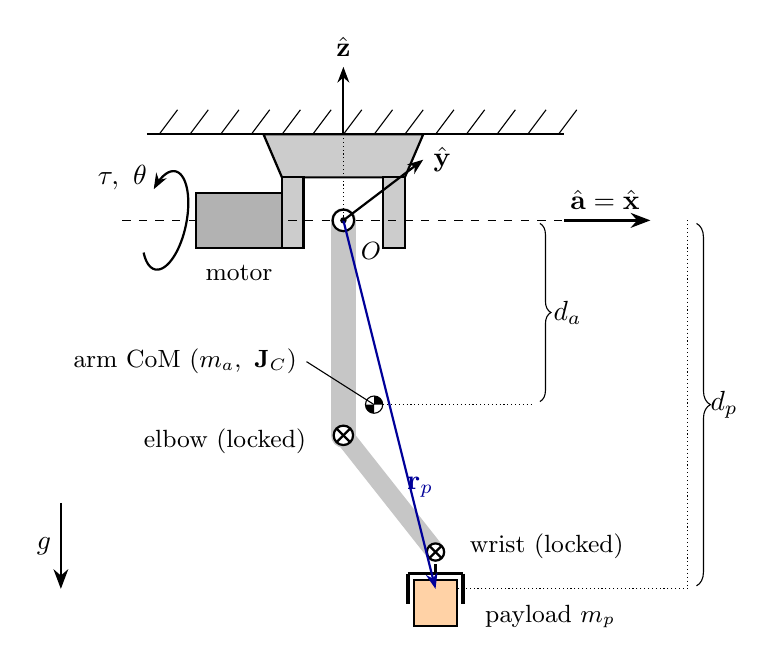
\begin{tikzpicture}[scale=0.78,
    x={(1cm,0cm)}, y={(0.5cm,0.38cm)}, z={(0cm,1cm)}]
    % 3D coordinates (x,y,z): x along the shoulder axis, z up; shoulder O at the origin.
    % Drawing scale: 1 unit = 0.1 m.

    % --- Ceiling ---
    \draw[thick] (-3.2,0,1.4) -- (3.6,0,1.4);
    \foreach \hx in {-3.0,-2.5,...,3.5}
        \draw (\hx,0,1.4) -- (\hx+0.3,0,1.8);

    % --- Ceiling mount (yoke) ---
    \filldraw[fill=gray!40, draw=black, thick] (-1.3,0,1.4) -- (1.3,0,1.4) -- (1.0,0,0.7) -- (-1.0,0,0.7) -- cycle;
    \filldraw[fill=gray!40, draw=black, thick] (-1.0,0,0.7) rectangle (-0.65,0,-0.45);
    \filldraw[fill=gray!40, draw=black, thick] (0.65,0,0.7) rectangle (1.0,0,-0.45);

    % --- Shoulder axis ---
    \draw[dashed] (-3.6,0,0) -- (3.7,0,0);
    \draw[-{Stealth[length=2.5mm]}, very thick] (3.6,0,0) -- (5.0,0,0) node[above left] {$\hat{\mathbf{a}} = \hat{\mathbf{x}}$};

    % --- Shoulder motor (on the left end of the axis) ---
    \filldraw[fill=gray!60, draw=black, thick] (-2.4,0,-0.45) rectangle (-1.0,0,0.45);
    \node[font=\small] at (-1.7,0,-0.85) {motor};
    \draw[-{Stealth[length=2mm]}, thick] plot[domain=200:480, samples=60, variable=\t]
        ({-2.9},{0.75*cos(\t)},{0.75*sin(\t)});
    \node at (-3.6,0,0.7) {$\tau,\ \theta$};

    % --- Links ---
    \draw[line width=9pt, gray!45, line cap=round] (0,0,0) -- (0,0,-3.5);
    \draw[line width=7pt, gray!45, line cap=round] (0,0,-3.5) -- (1.5,0,-5.4);
    \draw[thick] (0,0,0) circle (0pt);

    % --- Joints ---
    \filldraw[fill=white, draw=black, thick] (0,0,0) circle (5pt);
    \fill (0,0,0) circle (1.5pt);
    \node[font=\small] at (0.45,0,-0.5) {$O$};
    \filldraw[fill=white, draw=black, thick] (0,0,-3.5) circle (4.5pt);
    \draw[thick] ($(0,0,-3.5)+(-3pt,-3pt)$) -- ($(0,0,-3.5)+(3pt,3pt)$);
    \draw[thick] ($(0,0,-3.5)+(-3pt,3pt)$) -- ($(0,0,-3.5)+(3pt,-3pt)$);
    \node[font=\small, anchor=east] at (-0.45,0,-3.6) {elbow (locked)};
    \filldraw[fill=white, draw=black, thick] (1.5,0,-5.4) circle (4pt);
    \draw[thick] ($(1.5,0,-5.4)+(-2.6pt,-2.6pt)$) -- ($(1.5,0,-5.4)+(2.6pt,2.6pt)$);
    \draw[thick] ($(1.5,0,-5.4)+(-2.6pt,2.6pt)$) -- ($(1.5,0,-5.4)+(2.6pt,-2.6pt)$);
    \node[font=\small, anchor=west] at (1.9,0,-5.3) {wrist (locked)};

    % --- Gripper and payload ---
    \draw[very thick] (1.5,0,-5.6) -- (1.5,0,-5.75);
    \draw[very thick] (1.05,0,-5.75) -- (1.95,0,-5.75);
    \draw[very thick] (1.05,0,-5.75) -- (1.05,0,-6.25);
    \draw[very thick] (1.95,0,-5.75) -- (1.95,0,-6.25);
    \filldraw[fill=orange!35, draw=black, thick] (1.15,0,-5.85) rectangle (1.85,0,-6.6);
    \node[font=\small, anchor=west] at (2.15,0,-6.45) {payload $m_p$};

    % --- Arm CoM ---
    \coordinate (CA) at (0.5,0,-3);
    \filldraw[fill=white] (CA) circle (4pt);
    \fill (CA) -- ++(4pt,0) arc (0:90:4pt) -- cycle;
    \fill (CA) -- ++(-4pt,0) arc (180:270:4pt) -- cycle;
    \draw[thin] (CA) -- (-0.6,0,-2.3);
    \node[font=\small, anchor=east] at (-0.6,0,-2.3) {arm CoM ($m_a,\ \mathbf{J}_C$)};

    % --- Distance of the arm CoM from the axis ---
    \draw[densely dotted] (0.65,0,-3.0) -- (3.05,0,-3.0);
    \draw[decorate, decoration={brace, amplitude=4pt}] (3.2,0,-0.05) -- (3.2,0,-2.95);
    \node at (3.65,0,-1.5) {$d_a$};

    % --- Position vector of the payload and its distance from the axis ---
    \draw[-{Stealth[length=2mm]}, thick, blue!60!black] (0,0,0) -- (1.5,0,-6.0);
    \node[blue!60!black] at (1.25,0,-4.35) {$\mathbf{r}_p$};
    \draw[densely dotted] (5.6,0,0) -- (5.6,0,-6.0) -- (1.85,0,-6.0);
    \draw[decorate, decoration={brace, amplitude=5pt}] (5.75,0,-0.05) -- (5.75,0,-5.95);
    \node at (6.2,0,-3.0) {$d_p$};

    % --- Body axes at O ---
    \draw[-{Stealth[length=2mm]}, thick] (0,0,1.4) -- (0,0,2.5) node[above] {$\hat{\mathbf{z}}$};
    \draw[densely dotted] (0,0,0) -- (0,0,1.4);
    \draw[-{Stealth[length=2mm]}, thick] (0,0,0) -- (0,2.6,0) node[right] {$\hat{\mathbf{y}}$};

    % --- Gravity ---
    \draw[-{Stealth[length=2.5mm]}, thick] (-4.6,0,-4.6) -- (-4.6,0,-6.0);
    \node[left] at (-4.6,0,-5.3) {$g$};
\end{tikzpicture}
\caption{A ceiling-mounted robot arm, shown at $\theta = 0$ (hanging straight down). All joints except the shoulder are locked, so the arm and payload rotate together about the horizontal shoulder axis $\hat{\mathbf{a}}$ through $O$, driven by the shoulder motor torque $\tau$. The body frame is attached at $O$ with $\hat{\mathbf{x}}$ along the shoulder axis and $\hat{\mathbf{z}}$ pointing up at $\theta = 0$. The distances $d_a$ and $d_p$ are measured perpendicular to the shoulder axis. Drawing not to scale.}
\label{fig:robot}
\end{figure}

\noindent A robot arm is mounted from the ceiling, as shown in Fig.~\ref{fig:robot}. To check the sizing of its shoulder motor, we lock every joint with its brake except the top-most one (the shoulder), where the arm attaches to its ceiling mount. The arm and the payload in its gripper then move together as a single rigid body that can only rotate about the shoulder axis. The shoulder axis is the horizontal unit vector $\hat{\mathbf{a}}$ through the point $O$. The shoulder motor applies a torque $\tau$ about $\hat{\mathbf{a}}$, and $\theta$ is the angle the arm has rotated about $\hat{\mathbf{a}}$, measured from the position in which it hangs straight down. Because of the wrist offset, the arm does not lie in a plane perpendicular to the shoulder axis, so $\hat{\mathbf{a}}$ is \emph{not} a principal axis of the arm.

We use a body frame with origin at $O$, $\hat{\mathbf{x}} = \hat{\mathbf{a}}$, and $\hat{\mathbf{z}}$ pointing up when $\theta = 0$. In body-frame components:
\begin{itemize}
    \item The \textbf{arm} (all links and locked joints, without the payload) has mass $m_a$, its center of mass is at $\mathbf{r}_a$, and its inertia matrix about its \emph{own center of mass} is $\mathbf{J}_C$ (a full $3\times3$ matrix).
    \item The \textbf{payload} can be treated as a point mass $m_p$ at position $\mathbf{r}_p$.
\end{itemize}
When you need numbers in part (e), use $g = 9.81$~m/s$^2$ and
\[
\hat{\mathbf{a}} = \begin{bmatrix} 1 \\ 0 \\ 0 \end{bmatrix}, \qquad
m_a = 8~\text{kg}, \qquad
\mathbf{r}_a = \begin{bmatrix} 0.05 \\ 0 \\ -0.3 \end{bmatrix}\text{m}, \qquad
\mathbf{J}_C = \begin{bmatrix} 0.25 & 0.005 & 0.03 \\ 0.005 & 0.26 & 0.004 \\ 0.03 & 0.004 & 0.03 \end{bmatrix}\text{kg\,m}^2,
\]
\[
m_p = 2~\text{kg}, \qquad
\mathbf{r}_p = \begin{bmatrix} 0.15 \\ 0 \\ -0.6 \end{bmatrix}\text{m}, \qquad
d_a = 0.3~\text{m}, \qquad
d_p = 0.6~\text{m}.
\]

\exampagebreak

\begin{enumerate}[label=(\alph*)]

\item \pts{5} \textbf{Kinematics.} Write the arm's angular velocity $\bw$ and the velocities of the arm's center of mass, $\mathbf{v}_a$, and of the payload, $\mathbf{v}_p$, in terms of $\dot\theta$, $\hat{\mathbf{a}}$, $\mathbf{r}_a$, and $\mathbf{r}_p$.
\answerspace{2.6in}

\item \pts{10} \textbf{Kinetic energy.} Show that the total kinetic energy of the arm and payload is $T = \tfrac12 J_a\,\dot\theta^2$, and find an expression for $J_a$ in terms of $\mathbf{J}_C$, $m_a$, $m_p$, $d_a$, $d_p$, and $\hat{\mathbf{a}}$.
\answerspace{4.6in}
\exampagebreak

\item \pts{5} \textbf{Potential energy.} Write the gravitational potential energy $U(\theta)$ of the arm and payload.
\answerspace{2.6in}

\item \pts{8} \textbf{Equation of motion.} Form the Lagrangian and use the Euler--Lagrange equation with the generalized force $Q_\theta = \tau$ to find the equation of motion of the system.
\answerspace{4.2in}
\exampagebreak

\item \pts{7} \textbf{Sizing the shoulder motor.} What motor torque is needed to \textbf{hold} the payload stationary with the arm horizontal ($\theta = 90^\circ$)? What fraction of this torque is needed to support the arm itself, rather than the payload? Write your numerical answers with at least two significant digits of accuracy.
\answerspace{5.5in}

\end{enumerate}

% ==================================================================
\newpage
\section*{Part III: Explorer 1 and the Major-Axis Rule \hfill (35 points)}
% ==================================================================

\begin{figure}[h]
\centering
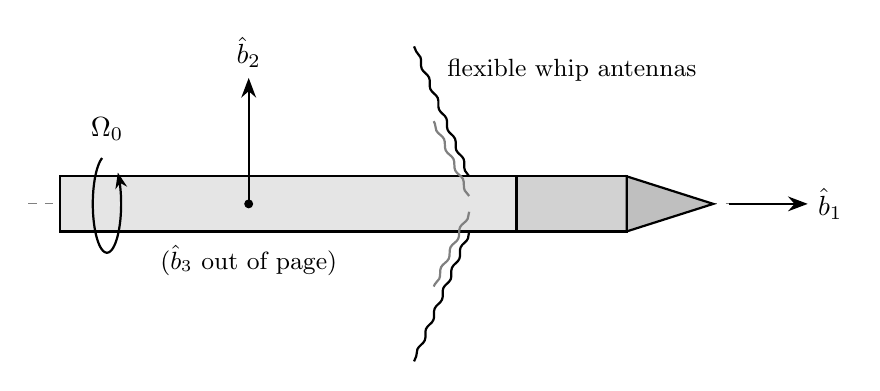
\begin{tikzpicture}[scale=1.0]
    % --- Spin axis (long axis, b1) ---
    \draw[dashed, gray] (-4.6,0) -- (4.9,0);
    \draw[-{Stealth[length=2.5mm]}, thick] (4.3,0) -- (5.3,0) node[right] {$\hat b_1$};

    % --- Rocket-stage body (long cylinder) ---
    \filldraw[fill=gray!20, draw=black, thick] (-4.2,-0.35) rectangle (1.6,0.35);
    % instrument section and nose cone
    \filldraw[fill=gray!35, draw=black, thick] (1.6,-0.35) rectangle (3.0,0.35);
    \filldraw[fill=gray!50, draw=black, thick] (3.0,-0.35) -- (4.1,0) -- (3.0,0.35) -- cycle;

    % --- Four whip antennas around the middle (two visible in profile, two foreshortened) ---
    \draw[thick, decorate, decoration={snake, amplitude=0.6pt, segment length=8pt}] (1.0,0.35) -- (0.3,2.0);
    \draw[thick, decorate, decoration={snake, amplitude=0.6pt, segment length=8pt}] (1.0,-0.35) -- (0.3,-2.0);
    \draw[thick, gray, decorate, decoration={snake, amplitude=0.6pt, segment length=8pt}] (1.0,0.1) -- (0.55,1.05);
    \draw[thick, gray, decorate, decoration={snake, amplitude=0.6pt, segment length=8pt}] (1.0,-0.1) -- (0.55,-1.05);
    \node[font=\small, anchor=west] at (0.6,1.7) {flexible whip antennas};

    % --- Spin about the long axis ---
    \draw[-{Stealth[length=2mm]}, thick] plot[domain=110:400, samples=60, variable=\t]
        ({0.18*cos(\t)-3.6},{0.62*sin(\t)});
    \node at (-3.6,0.95) {$\Omega_0$};

    % --- Transverse axes ---
    \draw[-{Stealth[length=2.5mm]}, thick] (-1.8,0) -- (-1.8,1.6) node[above] {$\hat b_2$};
    \filldraw (-1.8,0) circle (1.4pt);
    \node[below, font=\small, align=center] at (-1.8,-0.4) {($\hat b_3$ out of page)};
\end{tikzpicture}
\caption{Simplified sketch of Explorer 1. The satellite was spun about its long axis $\hat b_1$.}
\label{fig:explorer}
\end{figure}

\noindent Explorer 1, the first U.S.\ satellite, was launched on January 31, 1958. It was a long, slender cylinder, and it was spun about its \emph{long} axis at roughly 100~rad/s to keep its orientation steady. Within its first orbit, ground stations saw its radio signal change in a way that showed the satellite was no longer spinning about its long axis: it had gone into a \emph{flat spin}, tumbling end over end. The culprit turned out to be the four flexible whip antennas, which flexed slightly as the satellite wobbled and dissipated a tiny amount of energy. In this problem, you'll explain why that small amount of energy loss was enough to flip the satellite.

Model the satellite as a rigid body with principal moments of inertia $J_1, J_2, J_3$ about its CoM, with body axes $\hat b_i$ along the principal axes and $\hat b_1$ along the long axis. There are no external torques. When you need numbers in parts (b) and (d), use this simplified axisymmetric model:
\[
J_1 = J_a = 0.05~\text{kg\,m}^2, \qquad J_2 = J_3 = J_t = 3.0~\text{kg\,m}^2, \qquad \Omega_0 = 100~\text{rad/s}.
\]

\begin{enumerate}[label=(\alph*)]

\exampagebreak
\item \pts{5} \textbf{Euler's equations.} Start from ${}^{N}\dot{\bh} = \mathbf{0}$ and use the velocity-transport theorem to write the torque-free Euler equations for the body-frame components $\omega_1, \omega_2, \omega_3$. Without solving them, state two scalar quantities that are conserved for a torque-free \emph{rigid} body.
\answerspace{5.0in}
\exampagebreak

\item \pts{9} \textbf{Linear stability of pure spin.} Consider steady spin about the $\hat{b}_1$ axis, $\bw = (\Omega, 0, 0)$, and perturb it: $\bw = (\Omega + \delta_1,\ \delta_2,\ \delta_3)$ with small $\delta_i$.
\begin{enumerate}[label=(\roman*)]
    \item Linearize Euler's equations. Show that $\delta_1$ is constant to first order, and find linear ODEs for $\delta_2$ and $\delta_3$.
\answerspace{2.8in}
    \item For which orderings of $J_1, J_2, J_3$ is spin about the $\hat{b}_1$ axis linearly stable? State the result as a rule about the major, intermediate, and minor axes.
\answerspace{1.6in}
    \item Apply this to Explorer 1. Is spin about its long axis predicted to be stable? Find the frequency of the small wobble (in the body frame) in terms of $J_a$, $J_t$, and $\Omega$.
\answerspace{2.0in}
\end{enumerate}
\exampagebreak

\item \pts{9} \textbf{Energy at fixed angular momentum.} Now suppose that small internal motions (the flexing antennas) dissipate energy. These motions are internal, so they exert no net external torque.
\begin{enumerate}[label=(\roman*)]
    \item Explain why $\bh$ is still conserved but $T$ is not.
\answerspace{1.6in}
    \item Write $T$ in terms of the body-frame components of angular momentum $h_i = J_i\omega_i$. In terms of a fixed $\lVert\bh\rVert$, write down the maximum and minimum values of $T$.
\answerspace{2.4in}
    \item Use this to explain why pure spin about the minor axis cannot persist when there is any energy dissipation, however small, while spin about the major axis can. Why did the rigid-body analysis in part (b) give the wrong answer for Explorer 1?
\answerspace{2.4in}
\end{enumerate}
\exampagebreak

\item \pts{8} \textbf{The flat spin, by the numbers.} Using the model values above:
\begin{enumerate}[label=(\roman*)]
    \item Compute $\lVert\bh\rVert$ and the initial kinetic energy $T_0$.
\answerspace{1.6in}
    \item After the transition, Explorer 1 spins about a transverse axis. Find the final spin rate (in rad/s) and the final kinetic energy $T_f$.
\answerspace{2.0in}
    \item What fraction of the initial kinetic energy was dissipated? If the transition took about one 90-minute orbit, estimate the average power dissipated by the antennas.
\answerspace{2.0in}
\end{enumerate}
\exampagebreak

\item \pts{4} \textbf{Design lesson.} Suggest two design changes that would have kept Explorer 1 spinning stably.
\answerspace{4.0in}

\end{enumerate}

\end{document}
